A neuron is made of several fundamental components, crucial to build a meaningful model.
\begin{itemize}
    \item \textbf{Anatomical components:}
          \begin{itemize}
              \item Soma
              \item Dendrites
              \item Axons
              \item Spines
              \item Synapses
          \end{itemize}
    \item \textbf{Biophysical components:}
          \begin{itemize}
              \item Cell membranes
              \item Ion channels (Na\({}^{+}\), Ca\({}^{2+}\), K\({}^{+}\), Cl\({}^{-}\), \dots)
              \item Receptors
              \item Transporters
          \end{itemize}
    \item \textbf{Sub-cellular components:}
          \begin{itemize}
              \item Binding proteins
              \item Calcium stores
              \item Intracellular signaling cascades
          \end{itemize}
\end{itemize}
When it comes to computational problems there are mainly two approaches nowadays.
\begin{itemize}
    \item \textit{Abstract models:} the functioning of neurons is abstracted, while their morphology
          is disregarded.
          \begin{figure}[H]
              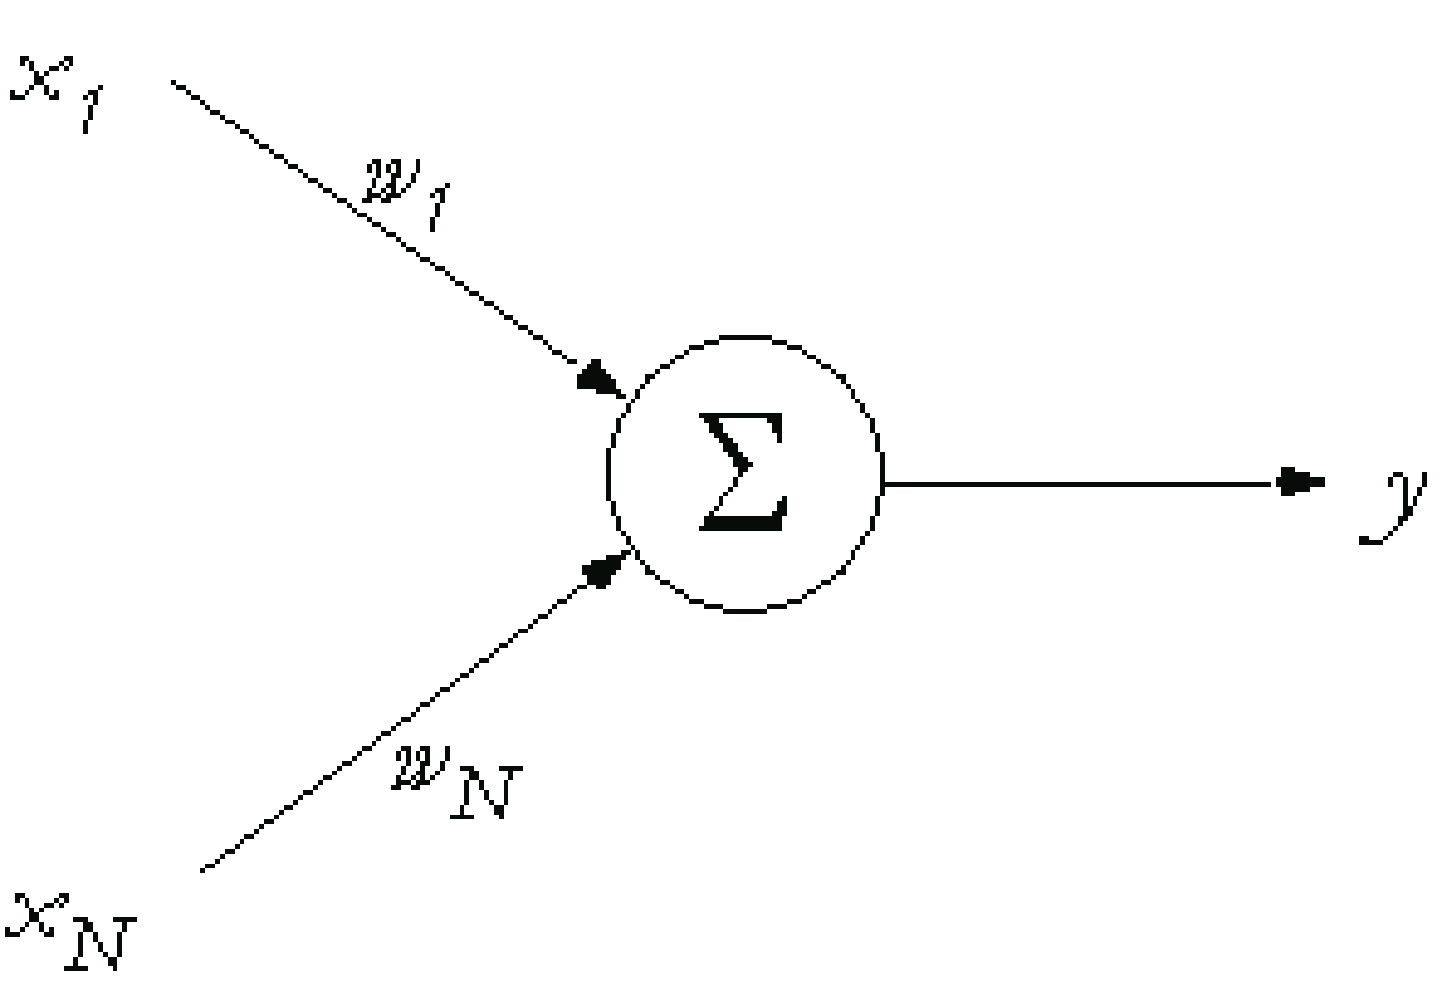
\includegraphics[scale=0.15]{02_1}
              \centering
          \end{figure}
    \item \textit{Realistic models:} the neurons morphology is kept into account as well, as it is
          considered a crucial characteristic for the model.
          \begin{figure}[H]
              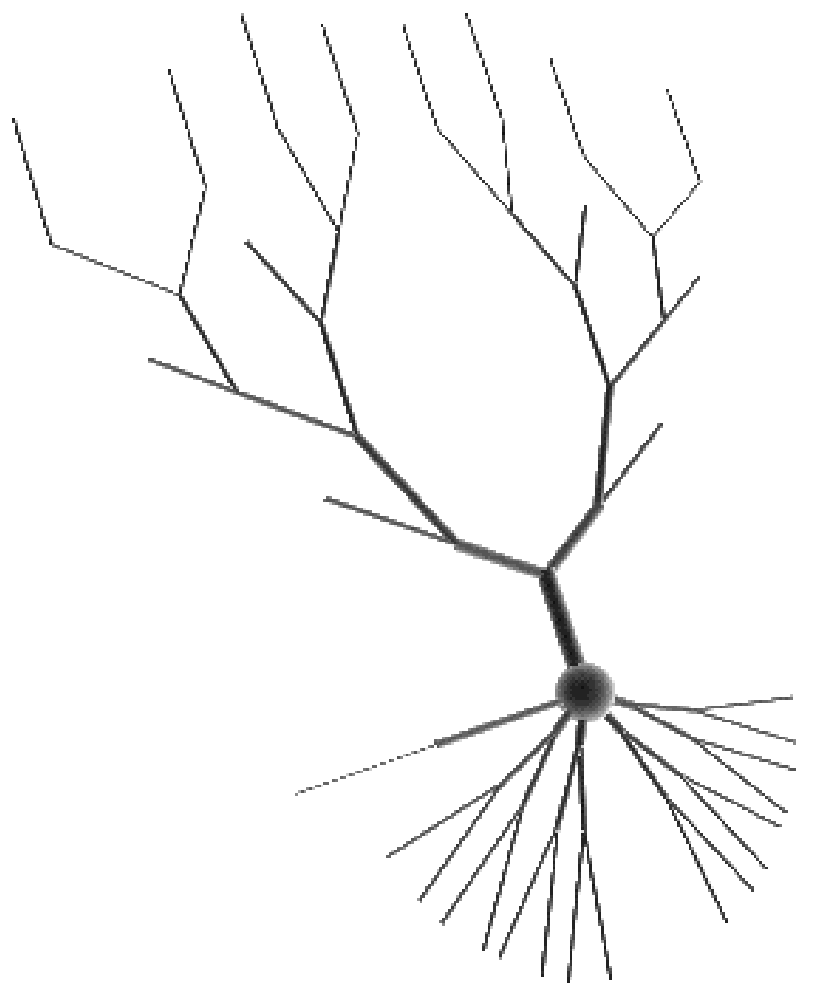
\includegraphics[scale=0.15]{02_2}
              \centering
          \end{figure}
\end{itemize}
\subsection{The Biophysical Structure of the Cell Membrane}
\paragraph{The Transmembrane Voltage}
When penetrating a neuron with a microelectrode, an electrical potential across the membrane is
measured. It is usually negative with respect to the ground (extracellular).
\begin{equation*}
    V_{m}(t)=V_{i}(t)-V_{e}(t)
\end{equation*}
The resting potential \(E_{rest}\), usually between \(-60\,mV\) and \(-70\,mV\), is the ordinary value for the
transmembrane voltage, when all the ionic currents are at the equilibrium and their net value is
zero.
\paragraph{The Transmembrane Capacitance}
A phospholipid bilayer separates the intracellular matrix from the extracellular one and it
separates ionic species, therefore it works as a capacitor, with negative charges inside the neuron
and positive charge on the outside surface:
\begin{equation*}
    Q=C_{m}\cdot V_{m}
    \hspace*{2.5cm}
    I_{C}=\frac{dQ}{dt}\Rightarrow
    I_{C}=C_{m}\frac{dV_{m}}{dt}
\end{equation*}
The membrane capacitance determines the membrane voltage dynamics, regulating how rapidly \(V_{m}\)
changes in response to a fixed current. The membrane capacitance is proportional to the surface area
of the cell, hence a specific membrane capacitance \(c_{m}\approx{1\,\mu{F}/cm^{2}}\) can be
introduced.
\paragraph{The Transmembrane Resistance}
The membrane displays voltage-independent channels with proteins allowing the leakage of ions
both into and out of the cell, iducing a current \(I_{leak}\). A leakage reversal potential
\(E_{m}\sim{E_{rest}}\) can thus be introduces. Then, the membrane voltage changes in a linear way,
following the Ohm's law:
\begin{equation*}
    V_{m}=R_{m}\cdot{I_{leak}}
\end{equation*}
where \(R_{m}\) is the transmembrane resistance. Notice that such a resistance is often
characterized by the related channel conductance \(g_{leak}=\frac{1}{R_{m}}\).\\
Holding the membrane potential steady at a level different from \(E_{rest}\) requires a certain
current, which is determined by the membrane (or input) resistance \(R_{m}\). Also in this
case it is possible to define the specific membrane resistance \(r_{m}\), independent on the
cell surface area.\\
\newline
To sum up, a neuron can be characterized by the measures reported in the picture below.
\begin{figure}[H]
    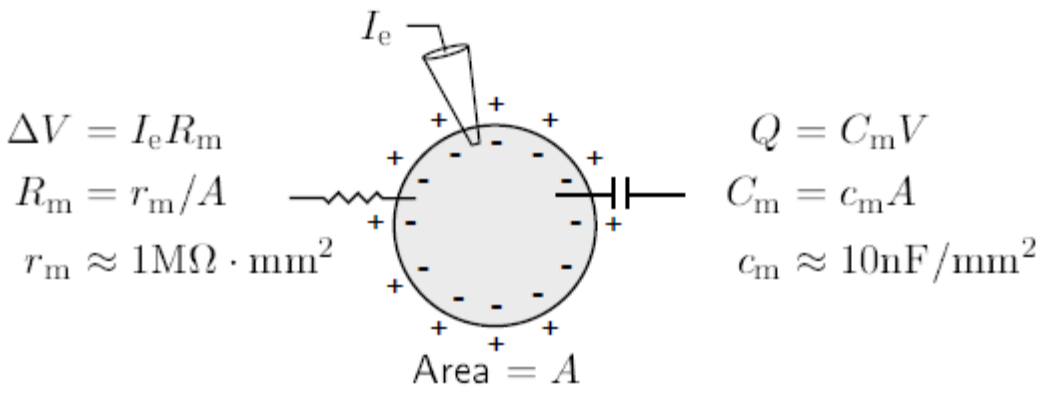
\includegraphics[scale=0.45]{02_3}
    \centering
\end{figure}
The membrane capacitance \(C_{m}\) and the membrane resistance \(R_{m}\) are employed to define
a membrane time constant \(\tau_{m}=R_{m}\cdot{C_{m}}=r_{m}\cdot{c_{m}}\) regulating the time
scale of changes in the membrane potential. It typically ranges in the \(10\,ms-100\,ms\) interval.\\
Now, the reported equivalent circuit can be derived from the previous considerations and the
relative KCL is shown just below it.
\begin{figure}[H]
    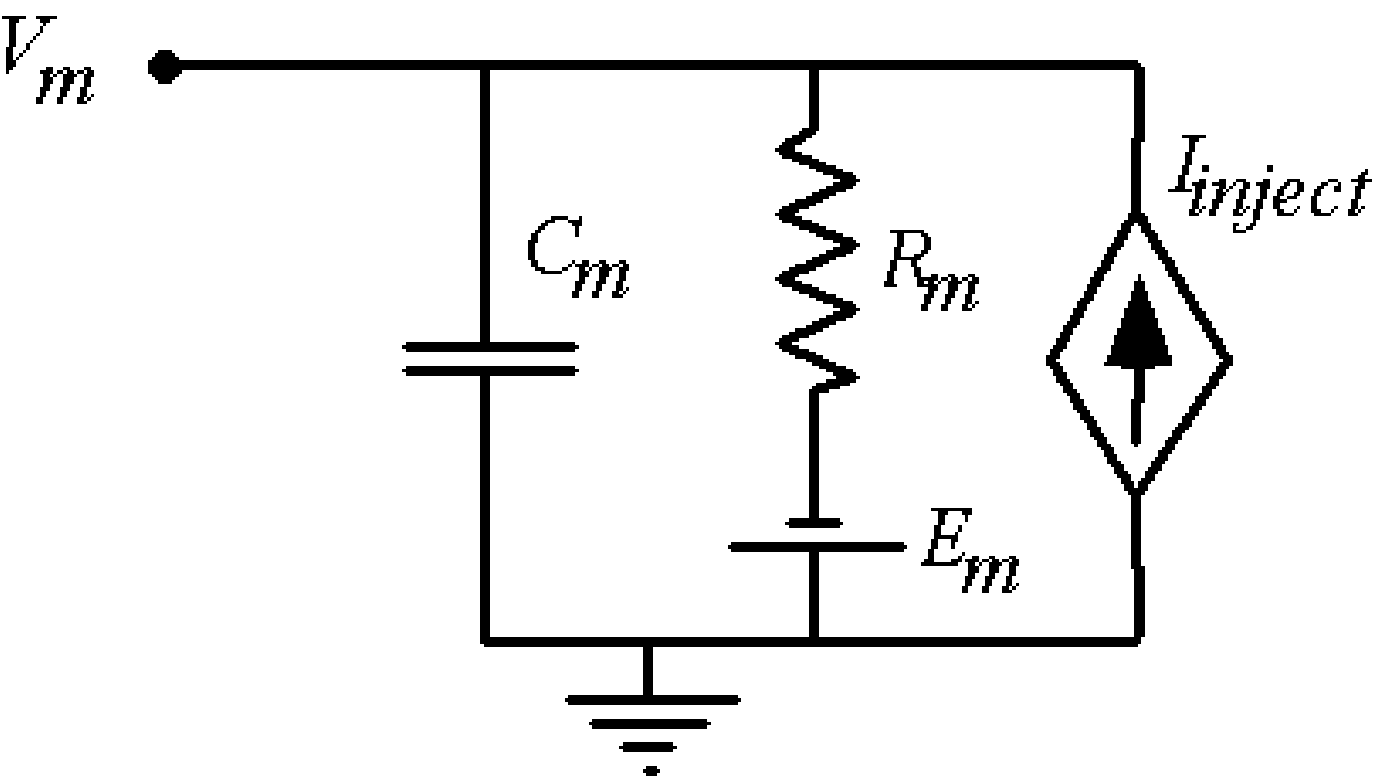
\includegraphics[scale=0.25]{02_4}
    \centering
\end{figure}
\begin{equation*}
    C_{m}\frac{dV_{m}}{dt}=-\frac{(V_{m}-E_{m})}{R_{m}}+I_{inject}
\end{equation*}
By solving the KCL, an expression for the membrane voltage as a function of time is obtained:
\begin{equation*}
    V_{m}(t)=V_{\infty}\bigl(1-e^{-\frac{t}{\tau_{m}}}\bigr)+E_{m}
\end{equation*}
\begin{equation*}
    \text{with}
    \hspace{0.25cm}
    V_{\infty}=R_{m}\cdot{I_{inject}}
    \hspace{0.25cm}
    \text{and}
    \hspace{0.25cm}
    \tau_{m}=R_{m}\cdot{C_{m}}
\end{equation*}
\subsection{Modelling the Single Channel}
So far, voltage-independent channels have been taken into account. However, cell membranes
contains a number of individual (voltage-dependent) channels. These channels open in a stochastic
way and their opening may be affected by several factors, such as the membrane potential \(V_{m}\),
intracellular ion concentration, and so on. Moreover, they are selective for one or more ions,
typically Na\({}^{+}\), K\({}^{+}\), Ca\({}^{2+}\), and Cl\({}^{-}\).
\begin{figure}[H]
    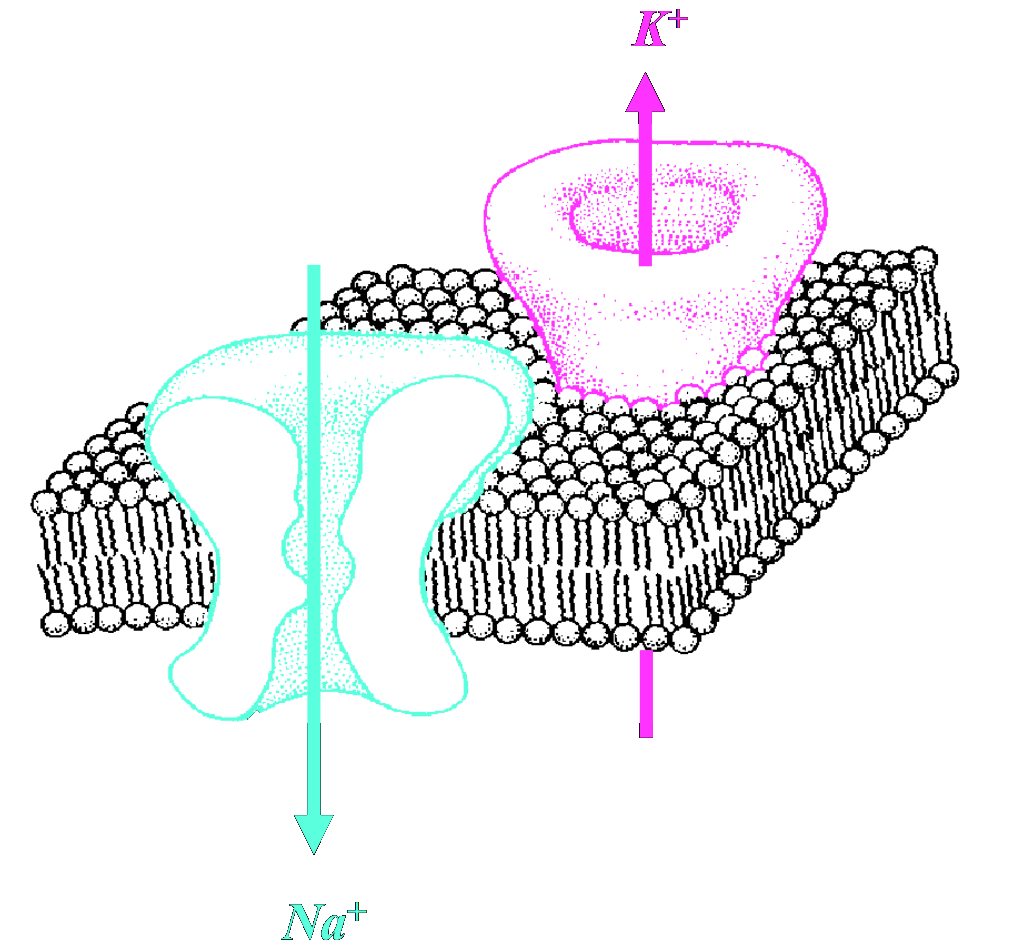
\includegraphics[scale=0.3]{02_5}
    \centering
\end{figure}
Whenever ions flow through these channels, some ionic currents \(I_{k}\) are generated. Generally,
\(I_{k}\) is related to the membrane voltage \(V_{m}\) through a linear relationship, leading
to the following equation.
\begin{equation*}
    I_{k}=g_{k}(V_{m}-E_{k})
\end{equation*}
Note that the conductance \(g_{k}\) is a function of several factors, in particular
\(g_{k}=f(V_{m},[k],t)\), with the ionic reversal potential \(E_{k}\) defined by the Nernst
equation as \(E_{k}=\frac{RT}{zF}\ln{\frac{[k]_{out}}{[k]_{in}}}\).\\
These voltage-dependent or concentration-dependent ionic currents can be incorporated in the
previously introduced equivalent circuit:
\begin{figure}[H]
    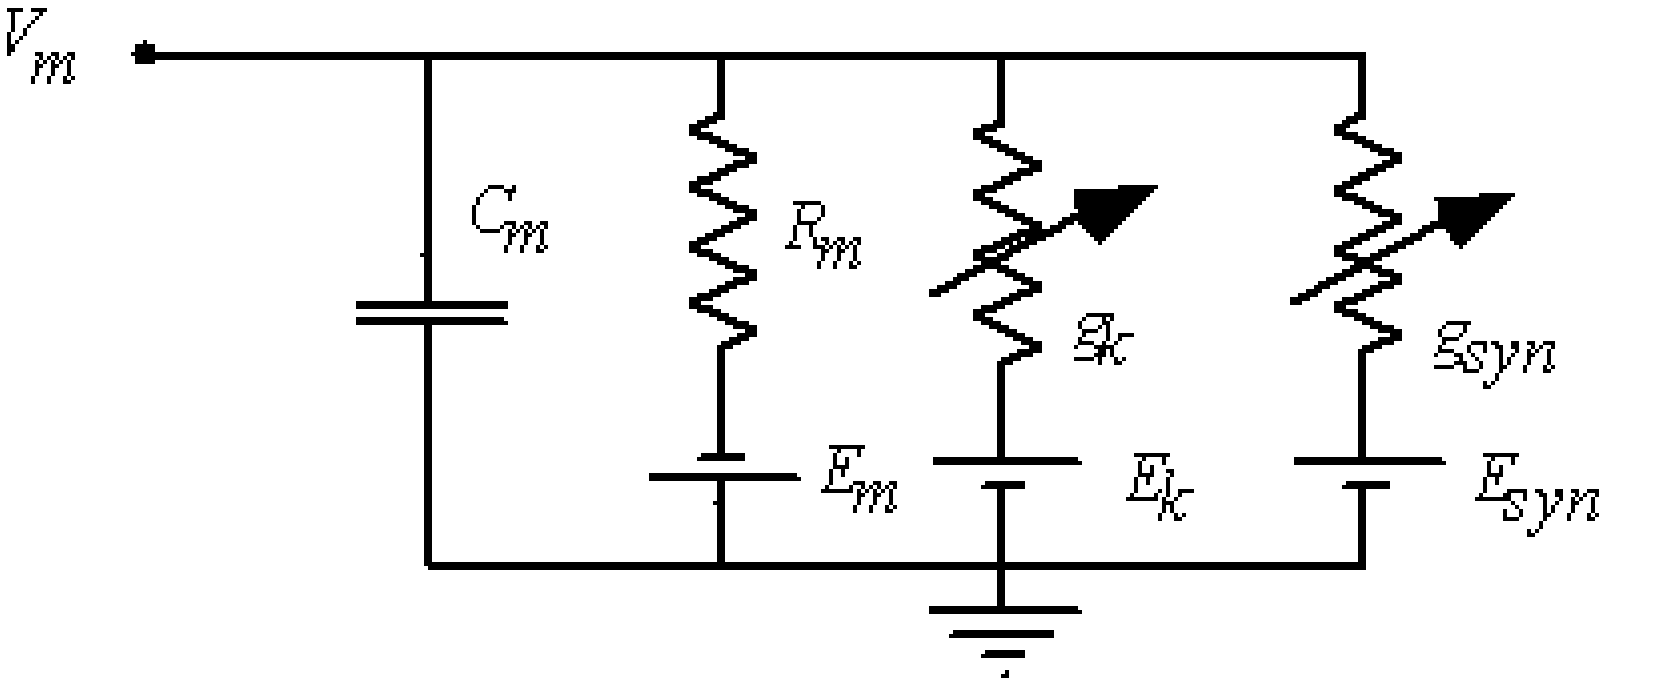
\includegraphics[scale=0.3]{02_6}
    \centering
\end{figure}
\begin{equation*}
    I_{k}=g_{k}(V_{m}-E_{k})
    \hspace{2.5cm}
    I_{syn}=g_{syn}(V_{m}-E_{syn})
\end{equation*}
Note that \(g_{syn}\) and \(E_{syn}\) are the synaptic conductance and the synaptic reversal
potential respectively.
\paragraph{Why are ionic channels modeled as resistive circuits?} The flux of ions through each
transmembrane ionic channel is ruled by both \textit{drift} and \textit{diffusion}. As a
consequence, they give birth to a drift-diffusion (ionic) current \(I_{k}\).
\begin{align*}
    I_{k}(x)
     & =I_{k,diffusion}(x)+I_{k,drift}(x)                      \\
     & =-z_{k}FD_{k}\frac{d[k](x)}{dx}+z_{k}F[k](x)\mu_{k}E(x)
\end{align*}
where \(E(x)\) is the electric field across the membrane.\\
By rearranging the equation, it can be obtained that:
\begin{equation*}
    \frac{I_{k}(x)}{\mu_{k}z_{k}F}=-\frac{D_{k}}{\mu_{k}}\frac{d[k](x)}{dx}+[k](x)E(x)
\end{equation*}
Note that due to the Einstein relationship \(\frac{D_{k}}{\mu_{k}}=\frac{RT}{z_{k}F}\), therefore:
\begin{equation*}
    \frac{I_{k}(x)}{\mu_{k}z_{k}F[k]}=
    -\frac{RT}{z_{k}F}\frac{1}{[k](x)}\frac{d[k](x)}{dx}-\frac{dV(x)}{dx}
\end{equation*}
Let's now integrate all the terms:
\begin{equation*}
    \int_{0}^{\Delta{x}}{\frac{I_{k}(x)}{\mu_{k}z_{k}F[k]}}dx=
    -\frac{RT}{z_{k}F}\int_{[k]_{in}}^{[k]_{out}}{\frac{1}{[k](x)}d[k](x)}
    -\int_{V_{in}}^{V_{out}}{dV(x)}
\end{equation*}
where \(\Delta{x}\) is the membranes thickness. At this point let's assume current density which
is constant across the membrane, such that it can be taken outside the integral.
\begin{equation*}
    I_{k}\int_{0}^{\Delta{x}}{\frac{1}{\mu_{k}z_{k}F[k]}}dx=
    -\frac{RT}{z_{k}F}\ln{\frac{[k]_{out}}{[k]_{in}}}
    -(V_{out}-V_{in})
\end{equation*}
Note that \(\int_{0}^{\Delta{x}}{\frac{1}{\mu_{k}z_{k}F[k]}}dx=R_{k}\), while
\(V_{in}-V_{out}=V_{m}\), leading to:
\begin{equation*}
    I_{k}{R_{k}}=V_{m}-E_{k}
\end{equation*}
This is the Ohm's law and this relationship has been derived without any assumption on the nature
of ionic channels or about their opening and closing dynamics.\\
Eventually, a crucial remark consists in saying that the electrophysiological properties of a
neuron are not exclusively caused by peculiar kinds of channels across its membrane. Also the
neuron morphology plays a fundamental role, thus it has to be modeled too.